\chapter{Experimenty}

\section{Jednoduchý příklad s batohem}
\begin{figure}[p]\centering
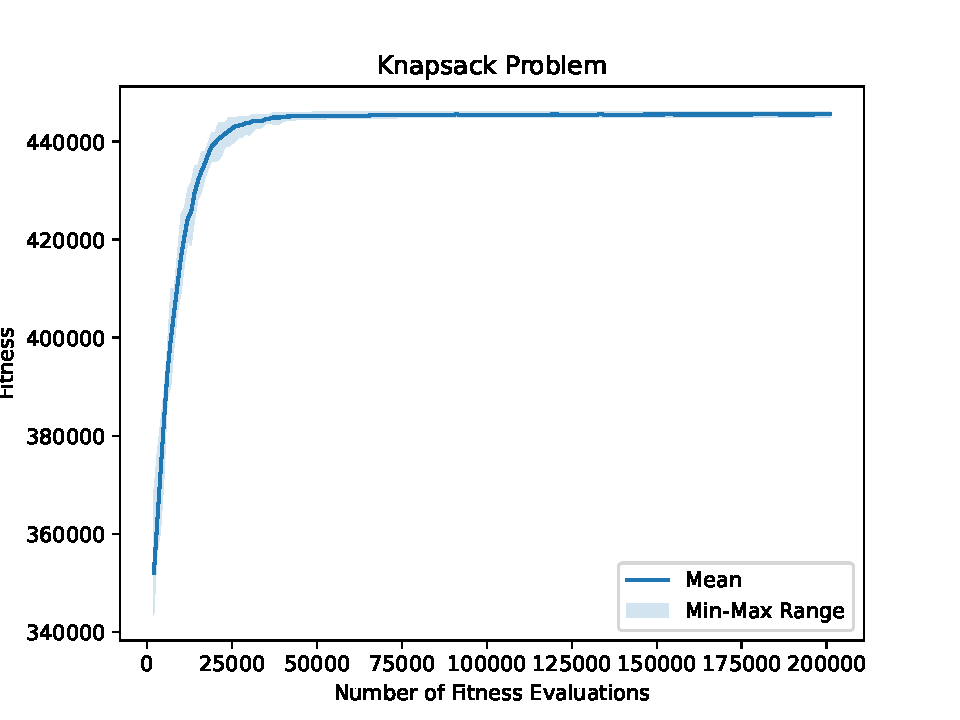
\includegraphics{img/knap}
\caption{Popisek?}
\label{exp:1}

\end{figure}


\section{Naivní přístup}
\begin{figure}[p]\centering
\includegraphics[width=\linewidth]{img/simple}
\caption{Popisek?}
\label{exp:2}
\end{figure}


\section{Agent s polárním kódováním}
\begin{figure}[p]\centering
\includegraphics[width=\linewidth]{img/polar}
\caption{Popisek?}
\label{exp:3}
\end{figure}


\section{Vylepšená fitness funkce}
\begin{figure}[p]\centering
\includegraphics[width=\linewidth]{img/impolar}
\caption{Popisek?}
\label{exp:4}
\end{figure}


\section{Populace s eliticismem}
\begin{figure}[p]\centering
\includegraphics[width=\linewidth]{img/elit}
\caption{Popisek?}
\label{exp:5}
\end{figure}


\section{Stěžující se fitness}
\begin{figure}[p]\centering
\includegraphics[width=\linewidth]{img/inc}
\caption{Popisek?}
\label{exp:6}
\end{figure}
